\begin{center}
    \textbf{Geração 100}
\end{center}

\begin{figure}[h]
    \centering
    \label{fig:geracao01}
    
    \begin{tabular}{rl}
        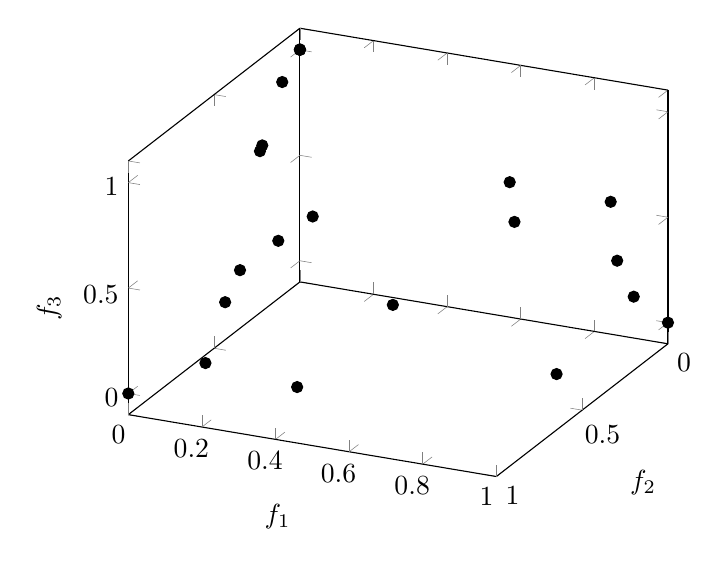
\begin{tikzpicture}[scale=1.0]
        	\begin{axis}[xlabel=$f_2$, ylabel=$f_1$, zlabel=$f_3$, view/h=115]
    			\addplot3[only marks] coordinates {
            		(1.000000, 0.000000, 0.000000) (0.000000, 1.000000, 0.000000) (0.000000, 0.000000, 1.000000) (0.000000, 0.000000, 1.000000) (0.000000, 0.000000, 1.002366) (0.705447, 0.581417, 0.405378) (0.320760, 0.732482, 0.601146) (0.219298, 0.672219, 0.707855) (0.631412, 0.329124, 0.703873) (0.906018, 0.414925, 0.093147) (0.818324, 0.218773, 0.534681) (0.490308, 0.120026, 0.863611) (0.883003, 0.208553, 0.420490) (0.134857, 0.924880, 0.356595) (0.007624, 0.847914, 0.533176) (0.194546, 0.042607, 0.982411) (0.965028, 0.193231, 0.179025) (0.435372, 0.900348, 0.001011) (0.724088, 0.278846, 0.632154) (0.468641, 0.116210, 0.876071) (0.136309, 0.970537, 0.200331) 

        		};
        	\end{axis}
	    \end{tikzpicture}
	    &
	    \begin{tikzpicture}[scale=1.0]
        	\begin{axis}[xlabel=$f_2$, ylabel=$f_1$, zlabel=$f_3$, view={45}{0}]
    			\addplot3[only marks] coordinates {
            		(1.000406,0.000000,0.000000)(0.000000,1.000821,0.000000)(0.000000,0.000000,1.000410)(0.000000,0.000000,1.000513)(0.000000,0.000000,1.008846)(0.428855,0.738966,0.536111)(0.376896,0.857096,0.353981)(0.060711,0.545878,0.837624)(0.577614,0.780391,0.241495)(0.648720,0.240773,0.740718)(0.500330,0.869753,0.178641)(0.771673,0.451443,0.449195)(0.871780,0.307549,0.387998)(0.975467,0.019472,0.228255)(0.027904,0.484476,0.875860)(0.231686,0.510675,0.829175)(0.490248,0.825942,0.289970)(0.828461,0.410978,0.383852)(0.212737,0.088363,0.975027)(0.730887,0.335500,0.608352)(0.483225,0.876988,0.015638) 

        		};
        	\end{axis}
	    \end{tikzpicture}
	\end{tabular}
    
\end{figure}

